\addcontentsline{toc}{part}{Day 1: Introductions and Overview of Rice Basics}
\part*{Day 1\\
Introductions and Overview of Rice Basics}
%% \phantomsection
\addcontentsline{toc}{section}{Exercise 1: Advanced Rice Customization Patterns}
{\setlength{\baselineskip}%
  {0.0\baselineskip}
  \section*{\flushright Exercise 1\\Advanced Rice Customization Patterns}
  \hrulefill \par}

\addcontentsline{toc}{subsection}{Description}
\subsection*{Description}
This exercise is designed to help developers explore different
patterns within Kuali Rice for development. There are many different
areas for customization within Rice itself. There are also just as
many different ways of doing the same thing. This can be confusing,
daunting, and troublesome. In this exercise, I will explore some
preferred methods for some advanced level customizations like creating
your own module within Rice or adding your own Constants to be
accessed from the webapp.
\addcontentsline{toc}{subsection}{Goals}
\subsection*{Goals}
\begin{itemize}
  \item Create a custom module.
  \item Create a custom DD Control class.
  \item See interesting ways to customize the portal.
  \item Create a custom JSP/JSTL function.
  \item Create a custom JstlListener and see how that works.
  \item Create custom parameters for your application-config.xml
    configuration
  \item Add an extension to a business object
\end{itemize}

\addcontentsline{toc}{subsection}{Creating a Custom Module}
\subsection*{1 Creating a Custom Module}

\subsection*{1.1 Browse the Rice Source Project}

\subsection*{1.2 Create a New Directory}
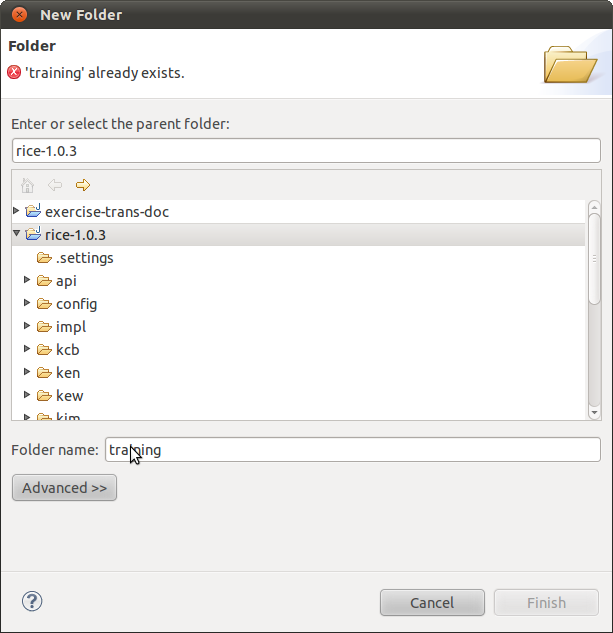
\includegraphics[width=\textwidth]{images/Screenshot.png}

Create a new directory in \emph{rice-src} called \emph{training}
\begin{lstlisting}[language=bash,basicstyle=\scriptsize,backgroundcolor=\color{ubergray},caption={Directory
    creation for Linux users},frame=single,breaklines=true]
mkdir training
\end{lstlisting}
In Eclipse, Refresh your project.

\subsection*{1.3 Add the Standard Structure}
\subsubsection*{1.3.1 Create Directories}
%% eclipse screenshot here
\begin{lstlisting}[language=bash,basicstyle=\scriptsize,backgroundcolor=\color{ubergray},caption={Directory creation for Linux
    users},frame=single,breaklines=true]
mkdir -p src/main/java/
mkdir -p src/main/resources/
mkdir -p src/main/config/
mkdir -p src/main/webapp/
mkdir -p src/test/java/
mkdir -p src/test/resources/
\end{lstlisting}
In Eclipse, Refresh your project.

\subsubsection*{1.3.1 Setup the Build Path}
In Eclipse:
\begin{enumerate}
  \item Expand the training folder
  \item Expand the src folder
  \item Expand the main folder
  \item Click your right mouse button on the java folder. A
    context menu will appear.
  \item Go to \textbf{Build Path} $\rightarrow$ \textbf{Use as Source
      Folder}
  \item Click your right mouse button on the resources folder. A
    context menu will appear.
  \item Go to \textbf{Build Path} $\rightarrow$ \textbf{Use as Source
      Folder}
  \item Expand the test folder
  \item Click your right mouse button on the test/java folder. A
    context menu will appear.
  \item Go to \textbf{Build Path} $\rightarrow$ \textbf{Use as Source
      Folder}
  \item Click your right mouse button on the test/resources folder. A
    context menu will appear.
  \item Go to \textbf{Build Path} $\rightarrow$ \textbf{Use as Source
      Folder}
  \item Click your right mouse button on the training folder. A
    context menu will appear.
  \item Go to \textbf{Build Path} $\rightarrow$ \textbf{Configure Build
      Path}
  \item A dialog will appear.\\
    \noindent 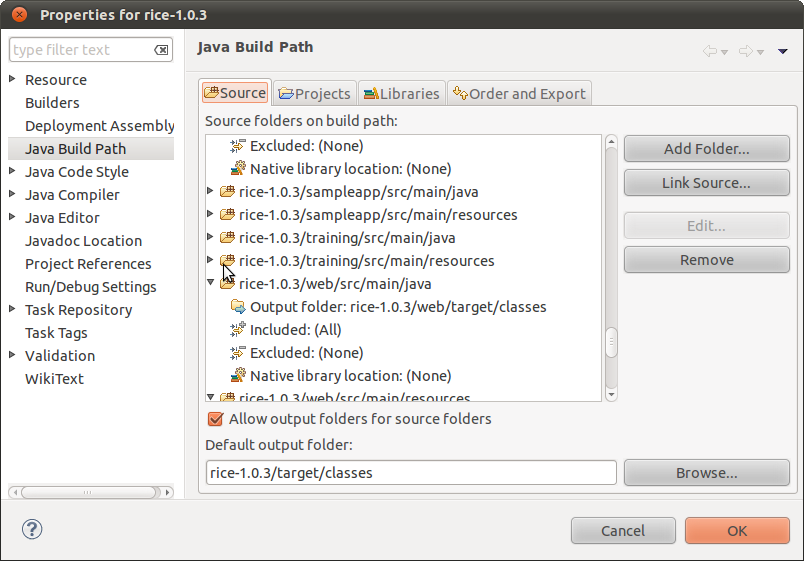
\includegraphics[width=\textwidth]{images/Screenshot3.png}
  \item Click on the \textbf{Source} tab.
  \item Locate rice-1.0.3/training build path configuration by scrolling
  \item Expand \textbf{training/src/main/java}
  \item Double-click on \textbf{Default output folder} next to the
    \textbf{Output Folder:}
  \item A dialog will appear.\\
    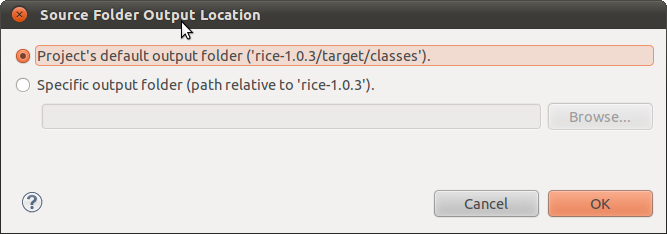
\includegraphics[width=\textwidth]{images/Screenshot4.png}

  \item Toggle \textbf{Specific output folder (path relative to
      'rice-1.0.3').}
  \item Enter \textbf{target/classes}
  \item Expand \textbf{training/src/main/resources}
  \item Double-click on \textbf{Default output folder} next to the
    \textbf{Output Folder:}
  \item A dialog will appear.
  \item Toggle \textbf{Specific output folder (path relative to
      'rice-1.0.3').}
  \item Enter \textbf{target/classes}
  \item Expand \textbf{training/src/test/java}
  \item Double-click on \textbf{Default output folder} next to the
    \textbf{Output Folder:}
  \item A dialog will appear.
  \item Toggle \textbf{Specific output folder (path relative to
      'rice-1.0.3').}
  \item Enter \textbf{target/test-classes}
  \item Expand \textbf{training/src/test/resources}
  \item Double-click on \textbf{Default output folder} next to the
    \textbf{Output Folder:}
  \item A dialog will appear.
  \item Toggle \textbf{Specific output folder (path relative to
      'rice-1.0.3').}
  \item Enter \textbf{target/test-classes}
\end{enumerate}


\subsection*{1.4 Create a pom.xml for the New Module}
\subsubsection*{1.4.1 Stub out training/pom.xml}
\begin{lstlisting}[numbers=left,language=xml,basicstyle=\scriptsize,backgroundcolor=\color{ubergray},caption={training/pom.xml},frame=single,breaklines=true]
<project xmlns="http://maven.apache.org/POM/4.0.0" xmlns:xsi="http://www.w3.org/2001/XMLSchema-instance" xsi:schemaLocation="http://maven.apache.org/POM/4.0.0 http://maven.apache.org/maven-v4_0_0.xsd">
  <name>Advanced Rice Training</name>
  <modelVersion>4.0.0</modelVersion>
  <parent>
    <groupId>org.kuali.rice</groupId>
    <artifactId>rice</artifactId>
    <version>1.0.3</version>
  </parent>
  <artifactId>training</artifactId>
  <packaging>war</packaging>
</project>
\end{lstlisting}

\subsubsection*{1.4.1 Add Basic Dependencies}
\begin{lstlisting}[numbers=left,language=xml,basicstyle=\scriptsize,backgroundcolor=\color{ubergray},caption={training/pom.xml},frame=single,breaklines=true]
  <dependencies>

    <dependency>
      <groupId>${project.groupId}</groupId>
      <artifactId>rice-impl</artifactId>
      <version>${project.version}</version>
    </dependency>

  </dependencies>  
\end{lstlisting}

\subsubsection*{1.4.2 Add the Maven Overlay Plugin}
\begin{lstlisting}[numbers=left,language=xml,basicstyle=\scriptsize,backgroundcolor=\color{ubergray},caption={training/pom.xml},frame=single,breaklines=true]
  <build>
    <plugins>
      <plugin>
        <groupId>org.apache.maven.plugins</groupId>
        <artifactId>maven-war-plugin</artifactId>
        <version>2.1.1</version>
        <configuration>
          <overlays>
            <overlay>
              <groupId>org.kuali.rice</groupId>
              <artifactId>rice-web</artifactId>
            </overlay>
          </overlays>
        </configuration>
      </plugin>
    </plugins>
  </build>
\end{lstlisting}

\subsubsection*{1.4.2 Add the Dependency to rice-web}
\begin{lstlisting}[numbers=left,language=xml,basicstyle=\scriptsize,backgroundcolor=\color{ubergray},caption={training/pom.xml},frame=single,breaklines=true]
    <dependency>
      <groupId>${project.groupId}</groupId>
      <artifactId>rice-web</artifactId>
      <version>${project.version}</version>
      <type>jar</type>
      <scope>compile</scope>
      <exclusions>
        <exclusion>
          <groupId>javax.servlet</groupId>
          <artifactId>servlet-api</artifactId>
        </exclusion>
        <exclusion>
          <groupId>javax.servlet</groupId>
          <artifactId>jstl</artifactId>
        </exclusion>
        <exclusion>
          <groupId>javax.servlet</groupId>
          <artifactId>jsp-api</artifactId>
        </exclusion>
      </exclusions>
    </dependency>

    <dependency>
      <groupId>${project.groupId}</groupId>
      <artifactId>rice-web</artifactId>
      <version>${project.version}</version>
      <type>war</type>
      <scope>runtime</scope>
      <exclusions>
        <exclusion>
          <groupId>javax.servlet</groupId>
          <artifactId>servlet-api</artifactId>
        </exclusion>
        <exclusion>
          <groupId>javax.servlet</groupId>
          <artifactId>jstl</artifactId>
        </exclusion>
        <exclusion>
          <groupId>javax.servlet</groupId>
          <artifactId>jsp-api</artifactId>
        </exclusion>
      </exclusions>
    </dependency>
\end{lstlisting}

\subsubsection*{1.4.3 Add the Tomcat Maven Plugin}
\begin{lstlisting}[numbers=left,language=xml,basicstyle=\scriptsize,backgroundcolor=\color{ubergray},caption={training/pom.xml},frame=single,breaklines=true]
      <plugin>
        <groupId>org.codehaus.mojo</groupId>
        <artifactId>tomcat-maven-plugin</artifactId>
        <!-- tomcat 6.0.26 -->
        <version>1.0</version>
        <configuration>
          <path>\$\{default.context.path\}</path>
        </configuration>
        <dependencies>
          <dependency>
            <groupId>mysql</groupId>
            <artifactId>mysql-connector-java</artifactId>
            <version>\$\{mysql.version\}</version>
            <scope>runtime</scope>
          </dependency>
        </dependencies>
      </plugin>
\end{lstlisting}

\subsubsection*{1.4.4 Add the Jetty Maven Plugin}
\begin{lstlisting}[numbers=left,language=xml,basicstyle=\scriptsize,backgroundcolor=\color{ubergray},caption={training/pom.xml},frame=single,breaklines=true]
      <plugin>
        <groupId>org.mortbay.jetty</groupId>
        <artifactId>jetty-maven-plugin</artifactId>
        <version>${jetty.version}</version>
        <configuration>
          <webAppConfig>
            <contextPath>${default.context.path}</contextPath>
          </webAppConfig>
        </configuration>
        <dependencies>
          <dependency>
            <groupId>mysql</groupId>
            <artifactId>mysql-connector-java</artifactId>
            <version>\$\{mysql.version\}</version>
            <scope>runtime</scope>
          </dependency>
        </dependencies>
      </plugin>					
\end{lstlisting}

\subsubsection*{1.4.5 Add the Maven Properties}
\begin{lstlisting}[numbers=left,language=xml,basicstyle=\scriptsize,backgroundcolor=\color{ubergray},caption={training/pom.xml},frame=single,breaklines=true
]
  <properties>
    <build.environment>dev</build.environment>
    <default.context.path>/\$\{project.artifactId\}--\${build.environment\}</default.context.path>
    <jetty.plugin.version>7.4.5.v20110725</jetty.plugin.version>
    <mysql.version>5.1.13</mysql.version>
  </properties>
\end{lstlisting}

\subsubsection*{1.4.6 Add the Maven Plugin Repositories}
\begin{lstlisting}[numbers=left,language=xml,basicstyle=\scriptsize,backgroundcolor=\color{ubergray},caption={training/pom.xml},frame=single,breaklines=true
]
  <pluginRepositories>
    <pluginRepository> 
      <id>kuali.nexus</id> 
      <name>Nexus Repository Manager</name> 
      <url>http://nexus.kuali.org/content/groups/public</url> 
      <releases> 
        <enabled>true</enabled> 
      </releases> 
      <snapshots> 
        <enabled>true</enabled> 
      </snapshots> 
    </pluginRepository>
  </pluginRepositories> 
\end{lstlisting}

\subsubsection*{1.4.6 Install rice-web.jar}
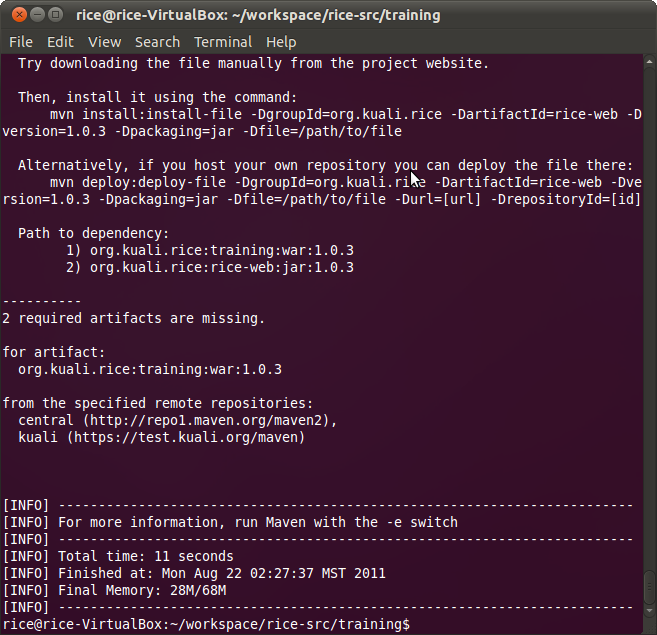
\includegraphics[width=\textwidth]{images/Screenshot6.png}
The above is what happens at this point if you try and install. The
rice-web.jar dependency cannot be fulfilled because it does not
exist. We need to create it.

\begin{lstlisting}[language=bash,basicstyle=\scriptsize,backgroundcolor=\color{ubergray},caption={Maven
  commands},frame=single,breaklines=true
]
cd /home/rice/workspace/rice-src/web
mvn -Dmaven.test.skip=true install
\end{lstlisting}

\begin{lstlisting}[language=bash,basicstyle=\scriptsize,backgroundcolor=\color{ubergray},caption={Maven
  commans},frame=single,breaklines=true
]
mvn jar:jar
\end{lstlisting}
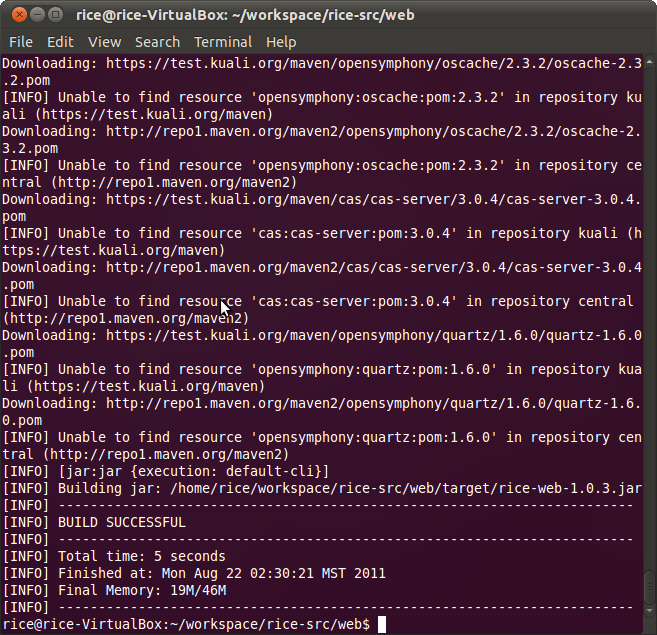
\includegraphics[width=\textwidth]{images/Screenshot7.png}

\begin{lstlisting}[language=bash,basicstyle=\scriptsize,backgroundcolor=\color{ubergray},caption={Maven
  commands},frame=single,breaklines=true
]
mvn install:install-file -DgroupId=org.kuali.rice
-DartifactId=rice-web -Dversion=1.0.3.2 -Dpackaging=jar -Dfile=target/rice-web-1.0.3.2.jar
\end{lstlisting}

\subsection*{1.5 Add a Base Package}
In Eclipse:
\begin{enumerate}
\item Click your right mouse button on the java folder. A context menu will appear.
\item Go to \textbf{New} $\rightarrow$ \textbf{Package}
\item A dialog will appear\\
  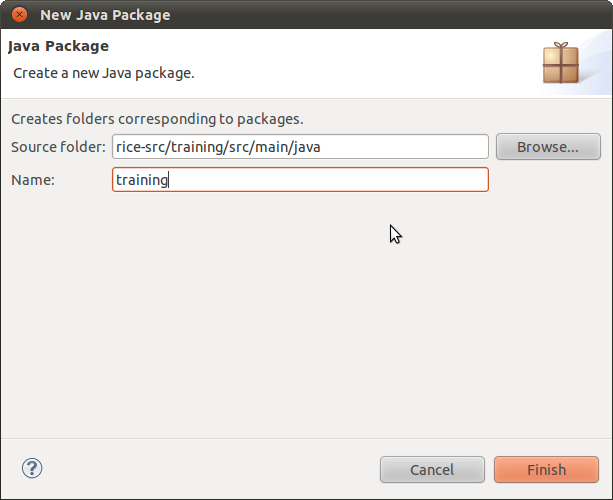
\includegraphics[width=\textwidth]{images/Screenshot9.png}
\item For Name, use \textbf{training}
\item Click Finish
\end{enumerate}

\subsection*{1.6 Create Base Spring Beans}
\subsubsection*{1.6.1 Stub out
  src/main/resources/training/SpringModuleBeans.xml}
\begin{lstlisting}[numbers=left,language=xml,basicstyle=\scriptsize,backgroundcolor=\color{ubergray},caption={Base
  SpringModuleBeans.xml},frame=single,breaklines=true]
<beans xmlns="http://www.springframework.org/schema/beans" xmlns:xsi="http://www.w3.org/2001/XMLSchema-instance" xmlns:aop="http://www.springframework.org/schema/aop" xmlns:tx="http://www.springframework.org/schema/tx"
	xsi:schemaLocation="http://www.springframework.org/schema/beans
                           http://www.springframework.org/schema/beans/spring-beans-2.0.xsd
                           http://www.springframework.org/schema/tx
                           http://www.springframework.org/schema/tx/spring-tx-2.0.xsd
                           http://www.springframework.org/schema/aop
                           http://www.springframework.org/schema/aop/spring-aop-2.0.xsd">
</beans>
\end{lstlisting}

\subsubsection*{1.6.1 Add the module bean with a parent}
\begin{lstlisting}[numbers=left,language=xml,basicstyle=\scriptsize,backgroundcolor=\color{ubergray},caption={Base
  SpringBeans.xml},frame=single,breaklines=true]

  <bean id="bookstoreModuleCconfiguration"
    parent="bookstoreModuleConfiguration-parentBean" />

  <bean id="bookstoreModuleConfiguration-parentBean" abstract="true"
     class="org.kuali.rice.kns.bo.ModuleConfiguration">
    <property name="namespaceCode" value="bookstore"/>
    <property name="initializeDataDictionary" value="true"/>
    <property name="dataDictionaryPackages">
      <list>
        <value>classpath:train/bookstore/bo/datadictionary/</value>
      </list>
    </property>
    <property name="databaseRepositoryFilePaths">
      <list>
	    <value>OJB-repository-bookstore.xml</value>
      </list>
    </property>
    <property name="packagePrefixes">
      <list>
        <value>train.bookstore.bo</value>
      </list>
    </property>
  </bean>
\end{lstlisting}

\subsubsection*{1.6.1 Add Spring datasource Configuration}
\begin{lstlisting}[basicstyle=\scriptsize,numbers=left,language=xml,backgroundcolor=\color{ubergray},caption={Spring
    datasource setup},frame=single,breaklines=true]
  <bean id="trainingDatasource" class="org.kuali.rice.core.database.PrimaryDataSourceFactoryBean" lazy-init="true">
    <property name="preferredDataSourceParams">
      <list>
        <value>training.datasource</value>
      </list>
    </property>
    <property name="preferredDataSourceJndiParams">
      <list>
        <value>training.datasource.jndi.location</value>
      </list>
    </property>
    <property name="serverDataSource" value="false"/>
  </bean>

  <bean id="trainingOjbConfigurer" class="org.kuali.rice.core.ojb.BaseOjbConfigurer">
    <property name="jcdAliases">
      <list>
        <value>trainingDataSource</value>
      </list>
    </property>
    <property name="metadataLocation" value="classpath:training/OJB-repository-bookstore.xml" />
  </bean>
\end{lstlisting}

\subsubsection*{1.6.1 Setup platformAwareDao}
\begin{lstlisting}[basicstyle=\scriptsize,numbers=left,language=xml,backgroundcolor=\color{ubergray},caption={Spring
    datasource setup src/main/resources/training/OJB-repository-bookstore.xml},frame=single,breaklines=true]
  <bean id="platformAwareDao" abstract="true" class="org.kuali.rice.kns.dao.impl.PlatformAwareDaoBaseOjb">
    <property name="jcdAlias" value="trainingDataSource" />
    <property name="dbPlatform" ref="dbPlatform" />
  </bean>
\end{lstlisting}

\subsection*{1.7 Stub Base OJB Mapping}
\begin{lstlisting}[basicstyle=\scriptsize,numbers=left,language=xml,backgroundcolor=\color{ubergray},caption={Stubbed
  OJB Descriptor file src/main/resources/OJB-repository-training.xml},frame=single,breaklines=true]
<descriptor-repository version="1.0">

  <jdbc-connection-descriptor jcd-alias="trainingDataSource" default-connection="false" jdbc-level="3.0" eager-release="false" batch-mode="false"
      useAutoCommit="0" ignoreAutoCommitExceptions="false">
    <sequence-manager className="org.kuali.rice.core.ojb.ConfigurableSequenceManager">
      <attribute attribute-name="property.prefix" attribute-value="datasource.ojb.sequenceManager" />
    </sequence-manager>
    <object-cache class="org.apache.ojb.broker.cache.ObjectCachePerBrokerImpl" />
  </jdbc-connection-descriptor>
</descriptor>
\end{lstlisting}

\addcontentsline{toc}{subsection}{Build It}
\subsection*{1.8 Build it}
\subsubsection*{1.8.1 Open a Shell to the Project Directory}
\begin{lstlisting}[basicstyle=\scriptsize,language=bash,backgroundcolor=\color{ubergray},caption={Change
  directory to the project in Linux},frame=single,breaklines=true]
cd workspace/rice-src/training
\end{lstlisting}
In Eclipse, Refresh your project.

\subsubsection*{1.8.2 Go}
\begin{lstlisting}[language=bash,basicstyle=\scriptsize,backgroundcolor=\color{ubergray},caption={Maven
  commands},frame=single,breaklines=true
]
cd /home/rice/workspace/rice-src/training
mvn -Dmaven.test.skip=true war:inplace
mvn -Dmaven.test.skip=true tomcat:run
\end{lstlisting}

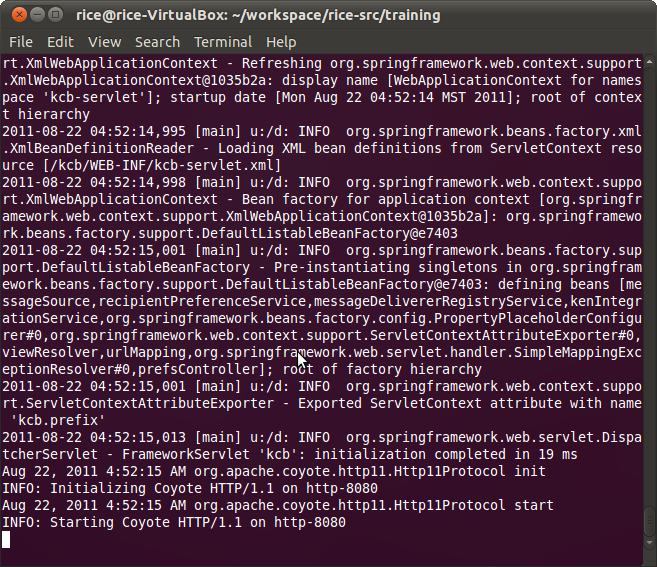
\includegraphics[width=\textwidth]{images/Screenshot10.png}
You should see the above after starting tomcat

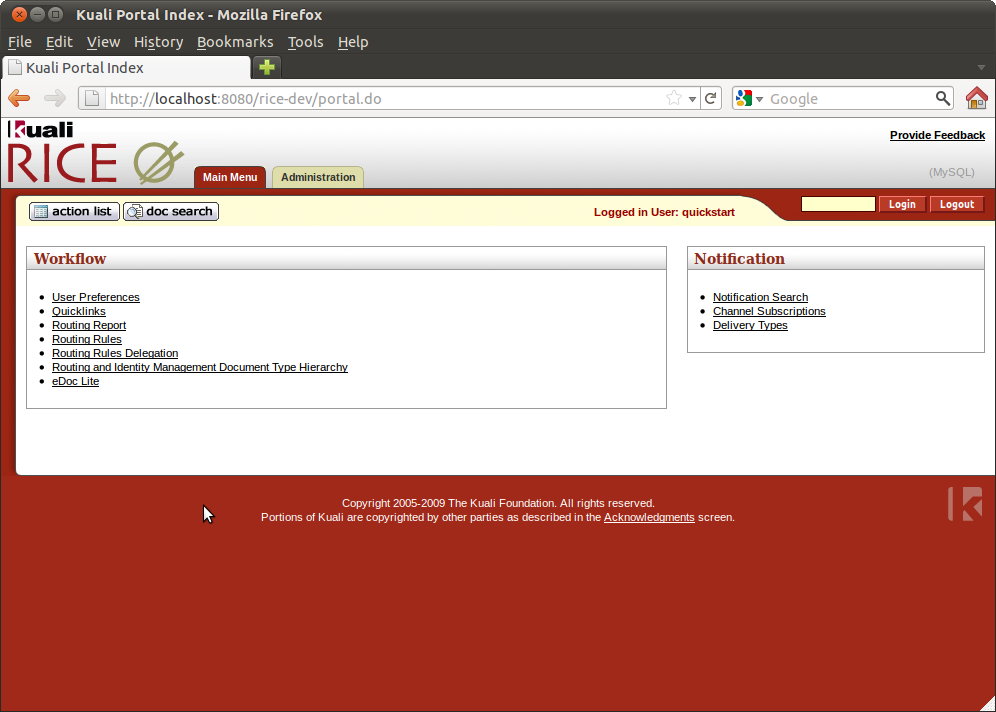
\includegraphics[width=\textwidth]{images/Screenshot11.png}
Browse to http://localhost:8080/rice-dev/. Then login as
quickstart. You should see the above.


\addcontentsline{toc}{subsection}{Creating a Custom Data Dictionary Control}
\subsection*{2 Creating a Custom Data Dictionary Control}
Control definitions are just Spring beans accessed via the
BusinessObjectMetadataService and the DataDictionaryService. Besides
controls, you can create or extend any aspect of the DataDictionary
including relationships, lookup definitions, and the workflow
attributes.

The core DataDictionary classes are located in
\textbf{impl/src/main/java/org/kuali/rice/kns/datadictionary/} of your
rice source code distribution.
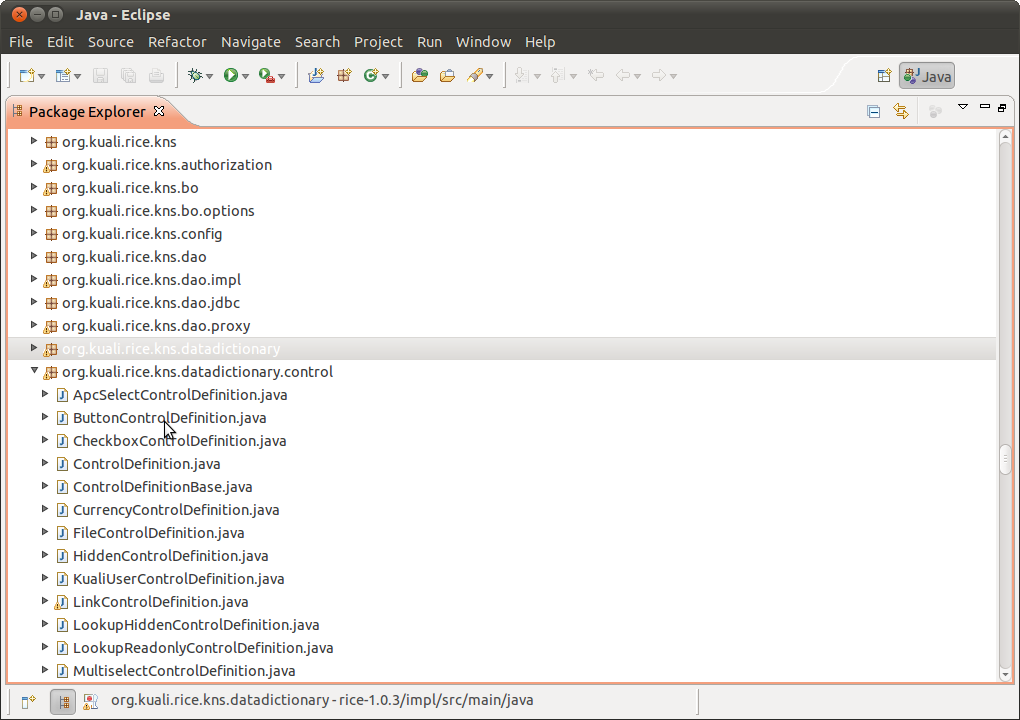
\includegraphics[width=\textwidth]{images/Screenshot-Java - Eclipse .png}

\subsubsection*{2.1 Add a datadictionary Package to Our Module}
%% Add an eclipse screenshot

\begin{lstlisting}[basicstyle=\scriptsize,language=bash,backgroundcolor=\color{ubergray},caption={Directory creation for Linux
    users},frame=single,breaklines=true]
  mkdir -p training/src/main/java/training/datadictionary/control
\end{lstlisting}

\emph{In Eclipse, Refresh your project.}

\subsubsection*{2.2 Stub SuggestsBox Control in src/main/java/training/datadictionary/control}
\begin{lstlisting}[basicstyle=\scriptsize,numbers=left,language=xml,backgroundcolor=\color{ubergray},caption={Stubbed
  OJB Descriptor file src/main/resources/OJB-repository-training.xml},frame=single,breaklines=true]
package training.datadictionary.control;

/**
 *
 */
public class SuggestsBoxDefinition extends ControlDefinitionBase {
    private static final long serialVersionUID = -1L;

	public SuggestsBoxDefinition() {
    }

    /**
     * @see java.lang.Object#toString()
     */
    public String toString() {
        return "SuggestsBoxDefinition";
    }
}
\end{lstlisting}

\addcontentsline{toc}{subsection}{Creating a Custom JSTL Function}
\subsection*{3 Creating a Custom JSTL Function}
\subsubsection*{3.1 Add a web Package to Our Module}
%% Add an eclipse screenshot

\begin{lstlisting}[basicstyle=\scriptsize,language=bash,backgroundcolor=\color{ubergray},caption={Directory creation for Linux
    users},frame=single,breaklines=true]
  mkdir -p training/src/main/java/training/web/
\end{lstlisting}

\subsubsection*{3.2 Stub a TrainingFunctions Class in the web
  Package}
\begin{lstlisting}[basicstyle=\scriptsize,numbers=left,language=java,backgroundcolor=\color{ubergray},caption={training/web/TrainingFunctions},frame=single,breaklines=true]
package training.web;

/**
 * Full of static methods for JSTL function access.
 * 
 */
public final class TrainingFunctions {
}
\end{lstlisting}

\subsubsection*{3.2 Add a Method that Fetches System Parameters}
\begin{lstlisting}[basicstyle=\scriptsize,numbers=left,language=java,backgroundcolor=\color{ubergray},caption={training/web/TrainingFunctions},frame=single,breaklines=true]
...
...
import static org.kuali.rice.kns.service.KNSServiceLocator.getParameterService

public final static boolean paramExists(final String component, final String
name) {
    return getParameterService().parameterExists("KR-TRN", component, name);
}

public final static String getParameter(final String component, final String
name) {
    return getParameterService().getParameterValue("KR-TRN", component, name);
}

public final static List<String> getParameters(final String component, final String
name) {
    return getParameterService().getParameterValues("KR-TRN", component, name);
}

public final static boolean isEnabled(final String component, final String
name) {
    return getParameterService().getIndicatorParameter("KR-TRN", component, name);
}
\end{lstlisting}

\subsubsection*{3.3 Stub a Tag Library Definition for the Module}
\begin{lstlisting}[basicstyle=\scriptsize,numbers=left,language=xml,backgroundcolor=\color{ubergray},caption={src/main/webapp/WEB-INF/tlds/trnfunc.tld
  Tag Library Definition},frame=single,breaklines=true]
<taglib xmlns="http://java.sun.com/xml/ns/j2ee" xmlns:xsi="http://www.w3.org/2001/XMLSchema-instance" xsi:schemaLocation="http://java.sun.com/xml/ns/j2ee http://java.sun.com/xml/ns/j2ee/web-jsptaglibrary_2_0.xsd" version="2.0">
</taglib>
\end{lstlisting}

\subsubsection*{3.4 Define the Tag Library}
\begin{lstlisting}[basicstyle=\scriptsize,numbers=left,language=xml,backgroundcolor=\color{ubergray},caption={src/main/webapp/WEB-INF/tlds/trnfunc.tld
  Tag Library Definition},frame=single,breaklines=true]
    <description>Training functions library</description>
    <display-name>Training functions</display-name>
    <tlib-version>1.0</tlib-version>
    <short-name>fn</short-name>
    <uri>http://www.kuali.org/jsp/jstl/functions</uri>
\end{lstlisting}

\subsubsection*{3.5 Add the Functions from TrainingFunctions}
\begin{lstlisting}[basicstyle=\scriptsize,numbers=left,language=xml,backgroundcolor=\color{ubergray},caption={src/main/webapp/WEB-INF/tlds/trnfunc.tld
  Tag Library Definition},frame=single,breaklines=true]
    <function>
        <description>Access System Parameters from JSTL</description>
        <name>parameterExists</name>
        <function-class>training.web.TrainingFunctions</function-class>
        <function-signature>boolean parameterExists(java.lang.String, java.lang.String)</function-signature>
        <example>&lt;c:if
        test="${trn-fn:parameterExists('Document', 'ACTIVE_FILE_TYPES')}"&gt;&lt;/c:if&gt;</example>
    </function>

    <function>
        <description>Access System Parameters from JSTL</description>
        <name>getParameter</name>
        <function-class>training.web.TrainingFunctions</function-class>
        <function-signature>java.lang.String getParameter(java.lang.String, java.lang.String)</function-signature>
        <example>${trn-fn:getParameter('Document', 'ACTIVE_FILE_TYPES')}</example>
    </function>

    <function>
        <description>Access System Parameters from JSTL</description>
        <name>getParameters</name>
        <function-class>training.web.TrainingFunctions</function-class>
        <function-signature>java.util.List getParameters(java.lang.String, java.lang.String)</function-signature>
        <example>${trn-fn:getParameters('Document', 'ACTIVE_FILE_TYPES')}</example>
    </function>

    <function>
        <description>Access System Parameters from JSTL</description>
        <name>isEnabled</name>
        <function-class>training.web.TrainingFunctions</function-class>
        <function-signature>boolean isEnabled(java.lang.String, java.lang.String)</function-signature>
        <example>${trn-fn:isEnabled('Document', 'ALLOW_NEGATIVE_BALANCE_IND')}</example>
    </function>
\end{lstlisting}

\subsubsection*{3.6 Test Yourself: What have you learned?}
Using the same examples above, add a call to \textbf{hasPermission} that
you can use to restrict a tab in the portal specifically for FO's.

\addcontentsline{toc}{subsection}{Adding to JstlConstantsInitListener}
\subsection*{3 Adding to JstlConstantsInitListener}
JstlConstantsInitListener can be found in
\textbf{impl/src/main/java/org/kuali/rice/kns/web/listener/JstlConstantsInitListener.java}
of your rice source distribution.
%% Eclipse screenshot here

\subsubsection*{3.1 Add a listener Package to Our Module}
%% Add an eclipse screenshot

\begin{lstlisting}[basicstyle=\scriptsize,language=bash,backgroundcolor=\color{ubergray},caption={Directory creation for Linux
    users},frame=single,breaklines=true]
  mkdir -p training/src/main/java/training/web/listener
\end{lstlisting}

\subsubsection*{3.1 Stub out a ContextListener}
\begin{lstlisting}[basicstyle=\scriptsize,numbers=left,language=java,backgroundcolor=\color{ubergray},caption={training/web/TrainingFunctions},frame=single,breaklines=true]
package training.web.listener;

import javax.servlet.ServletContext;
import javax.servlet.ServletContextEvent;
import javax.servlet.ServletContextListener;


/**
 * This class is the JstlContants implementation of the ServletContextListener.
 */
public class JstlConstantsInitListener implements ServletContextListener {
}
\end{lstlisting}


\subsubsection*{3.1 Add a Constant}
\begin{lstlisting}[basicstyle=\scriptsize,numbers=left,language=java,backgroundcolor=\color{ubergray},caption={training/web/TrainingFunctions},frame=single,breaklines=true]
package training;


import org.kuali.rice.core.util.JSTLConstants;

public class TrainingConstants extends JSTLConstants {
  public static String CURRENT_PROCESS_DATE_PARAMETER = "CURRENT_PROCESS_DATE";
}
\end{lstlisting}

\subsubsection*{3.1 Add Constants to the Listener}
\begin{lstlisting}[basicstyle=\scriptsize,numbers=left,language=java,backgroundcolor=\color{ubergray},caption={training/web/TrainingFunctions},frame=single,breaklines=true]
    import training.TrainingConstants;
    ...
    ...
    public void contextInitialized(ServletContextEvent sce) {

        ServletContext context = sce.getServletContext();
        // publish application constants into JSP app context with name "Constants"
        context.setAttribute("TrainingConstants", new TrainingConstants());
    }
\end{lstlisting}

\subsubsection*{3.1 Add the New InitListener to the web.xml}
The listener needs to be added to the Rice web.xml file. There is only
one web.xml file for an application. Each rice project has one. It
will be located in your project source tree at
src/main/webapp/WEB-INF/
%% Show Eclipse screenshot
 
In it, you will see a section with listeners that looks like:
\begin{lstlisting}[basicstyle=\scriptsize,numbers=left,language=java,backgroundcolor=\color{ubergray},caption={src/main/webapp/WEB-INF/web.xml},frame=single,breaklines=true]
    <listener>
      <listener-class>org.kuali.rice.core.web.listener.StandaloneInitializeListener</listener-class>
    </listener>

    <listener>
      <listener-class>org.kuali.rice.kns.web.listener.JstlConstantsInitListener</listener-class>
    </listener>

    <listener>
      <listener-class>org.kuali.rice.kns.web.listener.KualiHttpSessionListener</listener-class>
    </listener>
\end{lstlisting}

Just add yours. Now when your application starts, you will be able to
access your constants from the JSP/JSTL.

\addcontentsline{toc}{section}{Exercise 2: Portal Customization}
{\setlength{\baselineskip}%
  {0.0\baselineskip}
  \section*{\flushright Exercise 2\\Portal Customization}
  \hrulefill \par}

\addcontentsline{toc}{subsection}{Description}
\subsection*{Description}
Besides a middleware framework and API, Rice supplies a reference
implementation portal with administrative focused user
interfaces. Most institutions will want to customize this to fit their
users and their functional needs. That will involve some modification
at just about any level. This exercise explores advanced techniques
for portal customization

\addcontentsline{toc}{subsection}{Goals}
\subsection*{Goals}
\begin{itemize}
  \item Learn new ways to use javascript to communicate with SOA 
  \item How to creatively add functionality and rich user interface
    design to the Kuali Portal
\end{itemize}

\addcontentsline{toc}{subsection}{1 Add a new Tab Restricted by Permission}
\subsection*{1 Add a New Tab Restricted by Permission}

\addcontentsline{toc}{subsection}{2 Add Fancy Tooltips to Channel Content}
\subsection*{2 Add Tooltips to Channels}

\newpage
  {\setlength{\baselineskip}%
           {0.0\baselineskip}
  \section*{Notes}
  \hrulefill \par}

